\cleardoublepage % memastikan bab baru dimulai di halaman ganjil (kanan)

\chapter{STUDI LITERATUR}
\label{chap:studi-literatur}

\section{Arsitektur \textit{Cloud} Modern dan Tantangan Kompleksitas}

Aplikasi \textit{cloud-native} adalah perangkat lunak yang dirancang sejak awal untuk berjalan di lingkungan \textit{cloud} dengan memanfaatkan skalabilitas, resiliensi, dan elastisitas infrastruktur modern \parencite{soldani_pains_2018}. Pergeseran paradigma dari arsitektur monolitik menuju layanan mikro (\textit{microservices}) kini telah menjadi fondasi utama dalam pengembangan aplikasi \textit{cloud-native} modern. Berbeda dengan pendekatan arsitektur tradisional, gaya arsitektur layanan mikro mendistribusikan logika bisnis secara masif ke dalam puluhan hingga ratusan layanan kecil independen. Distribusi fungsionalitas ini memunculkan kebutuhan akan mekanisme \textit{deployment} independen. Sebagai solusi, layanan mikro secara alami terintegrasi dengan platform berbasis kontainer karena setiap layanan dapat dikemas dan didistribusikan di dalam kontainernya masing-masing \parencite{soldani_pains_2018}. Walaupun memberikan keuntungan operasional yang signifikan berupa portabilitas lintas \textit{cloud}, skalabilitas tingkat tinggi, dan kebebasan pemilihan teknologi bagi pengembang, ekosistem kontainer ini juga menghadirkan tantangan kompleksitas \parencite{soldani_pains_2018}.

Dalam lingkungan terdistribusi ini, setiap layanan berkomunikasi melalui antarmuka API yang bertindak sebagai kontrak standar komunikasi antarlayanan \parencite{soldani_pains_2018}. Kesalahan interpretasi terhadap arsitektur dan kontrak API ini sering kali berujung pada kegagalan operasional; kegagalan satu layanan dapat memicu rentetan kegagalan layanan lain yang bergantung padanya (\textit{cascading failures}) \parencite{soldani_pains_2018}. Akibatnya, dokumentasi API dan manifes konfigurasi orkestrasi menjadi semakin kompleks, yang menjadi tantangan utama pengembang \textit{cloud-native}.

\section{Kubernetes: Platform Orkestrasi Kontainer untuk Aplikasi \textit{Cloud-Native}}

Kubernetes merupakan platform orkestrasi kontainer yang dirancang untuk mengotomatisasi proses \textit{deployment}, \textit{scaling}, dan manajemen aplikasi berbasis kontainer dalam lingkungan \textit{cloud-native} \parencite{kubernetes_docs}. Platform ini menyediakan mekanisme deklaratif berbasis konfigurasi yang memungkinkan pengguna mendefinisikan keadaan sistem yang diinginkan (\textit{desired state}) melalui berkas konfigurasi, sementara Kubernetes menjaga agar keadaan tersebut tetap terpenuhi melalui rangkaian komponen pengendali (\textit{controller loops}).

\subsection{Gambaran Umum Arsitektur}

Arsitektur Kubernetes dibangun atas konsep klaster yang terdiri dari dua kelompok komponen utama, yaitu \textit{Control Plane} dan \textit{Worker Nodes}. \textit{Control Plane} berfungsi sebagai pengendali utama yang membuat keputusan bisnis aplikasi, misalnya penjadwalan, pemantauan, serta konsistensi status. \textit{Worker Nodes} merupakan mesin (server) fisik atau virtual yang menjalankan kontainer sebagai satuan aplikasi. Kedua komponen ini berkomunikasi secara internal melalui API server yang menjadi pintu utama seluruh permintaan sistem.

\begin{figure}[H]
    \centering
    \captionsetup{justification=centering}
    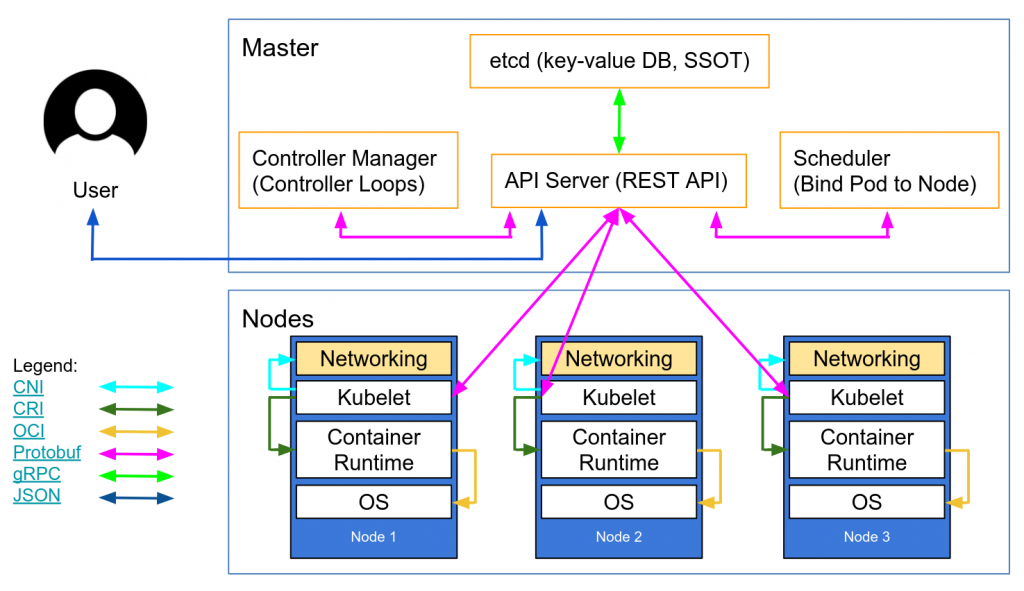
\includegraphics[width=1.00\textwidth]{images/arsi-kube.png}
    \caption{Arsitektur klaster Kubernetes yang terdiri atas \textit{Control Plane} dan \textit{Worker Nodes}, dihubungkan melalui \textit{kube-apiserver} \parencite{kubernetes_docs}}
    \label{fig:kubernetes-architecture}
\end{figure}

\begin{enumerate}
    \item \textbf{\textit{Control Plane}}\\
    \textit{Control Plane} bertanggung jawab mengelola keadaan (\textit{state}) klaster secara keseluruhan. Komponen utamanya meliputi,
    \begin{enumerate}[a.]
        \item \textbf{kube-apiserver} sebagai gerbang utama untuk mengelola objek Kubernetes melalui API,
        \item \textbf{etcd} sebagai basis data \textit{key-value} yang menyimpan informasi konfigurasi dan status,
        \item \textbf{kube-scheduler} yang menentukan Node penempatan Pod berdasarkan ketersediaan sumber daya,
        \item \textbf{kube-controller-manager} yang berisi sekumpulan kontroler untuk menjaga kesesuaian antara kondisi aktual dan \textit{desired state}. Melalui mekanisme deklaratif ini, Kubernetes secara otomatis memperbaiki status objek yang tidak sesuai dan memastikan setiap aplikasi berjalan sesuai aturan konfigurasi yang ditentukan.
    \end{enumerate}
    \item \textbf{\textit{Worker Nodes}}\\
    \textit{Worker Nodes} merupakan lapisan eksekusi tempat aplikasi berjalan dalam bentuk Pod. Node terdiri atas tiga komponen inti:
    \begin{enumerate}[a.]
        \item \textbf{kubelet} yang bertugas mengeksekusi Pod sesuai \textit{specification} yang diterima dari \textit{Control Plane},
        \item \textbf{kube-proxy} yang menyediakan layanan \textit{network forwarding} dan \textit{load balancing} sederhana antar-\textit{Pod} dalam klaster,
        \item \textbf{\textit{container runtime}} yang bertanggung jawab menjalankan kontainer. Dengan demikian, Node menjalankan komputasi terdistribusi yang dikontrol oleh \textit{Control Plane} melalui komunikasi berbasis API.
    \end{enumerate}
\end{enumerate}

\subsection{\textit{Resource Model} dan Hierarki}

Dalam \textit{resource model} Kubernetes, terdapat beberapa objek inti pembangun aplikasi yang paling sering digunakan:

\begin{enumerate}[a.]
    \item \textbf{\textit{Pod}}: Unit komputasi terkecil sebagai pembungkus kontainer aplikasi
    \item \textbf{\textit{Deployment}}: Pengatur replika dan proses pembaruan versi untuk mencapai \textit{high availability}
    \item \textbf{\textit{Service}}: Penyedia titik akses jaringan yang stabil untuk aplikasi di dalam \textit{Pod}
    \item \textbf{\textit{Ingress}}: Pengatur rute lalu lintas eksternal masuk ke dalam klaster
    \item \textbf{\textit{ConfigMap}}: Penyimpan variabel lingkungan dan konfigurasi non-sensitif
    \item \textbf{\textit{Secret}}: Pengelola data sensitif seperti kredensial dan token
    \item \textbf{\textit{PersistentVolumeClaim}}: \textit{Persistent storage} untuk data aplikasi yang bersifat \textit{stateful}
    \item \textbf{\textit{ServiceAccount}}: Identitas yang digunakan oleh \textit{Pod} untuk berinteraksi dengan API server
    \item \textbf{\textit{Role}} dan \textbf{\textit{RoleBinding}}: Kontrol akses berbasis peran (RBAC)
    \item \textbf{\textit{HorizontalPodAutoscaler}}: Pengatur skala otomatis berdasarkan metrik penggunaan
\end{enumerate}

Antarobjek ini saling terikat melalui berbagai jenis relasi semantik yang mencakup relasi kepemilikan (\textit{ownership}), ketergantungan fungsional (\textit{dependencies}), dan relasi konfigurasi.
\subsection{Manifes YAML dan \textit{Infrastructure as Code}}

Pengembang berinteraksi dengan model sumber daya Kubernetes melalui pendekatan \textit{Infrastructure as Code} (IaC) \parencite{k8s_docs_concepts}. Pendekatan ini mewajibkan pengguna untuk mendeklarasikan wujud infrastruktur yang diinginkan (\textit{desired state}) ke dalam bentuk dokumen teks berformat YAML. Setiap manifes YAML standar wajib memiliki empat atribut struktural utama agar dapat diterima oleh API Kubernetes:
\begin{enumerate}
    \item \texttt{apiVersion}: Menentukan versi skema API pembungkus objek.
    \item \texttt{kind}: Mendefinisikan jenis objek Kubernetes.
    \item \texttt{metadata}: Memuat data identifikasi unik seperti nama, label pengelompokan, dan \textit{namespace}.
    \item \texttt{spec}: Mendefinisikan \textit{desired state} atau kondisi yang diharapkan dari sebuah objek Kubernetes.
\end{enumerate}

Penyusunan manifes YAML menuntut pemahaman terkait batasan skema. Pengembang dituntut memahami perbedaan antara atribut wajib (\textit{required}) yang menentukan validitas manifes dan atribut opsional (\textit{optional}) yang memberikan fleksibilitas konfigurasi. Praktik terbaik dalam penulisan IaC menyarankan modularitas dokumen, konsistensi penggunaan label, dan pemisahan logika aplikasi dari data konfigurasi.

\section{\textit{Large Language Models} (LLM)}
\subsection{Definisi dan Kapabilitas}
\textit{Large Language Model} (LLM) merupakan model kecerdasan buatan berbasis jaringan saraf berskala besar yang dilatih pada korpus teks \textit{multi-domain} untuk mempelajari representasi bahasa alami secara mendalam \parencite{wan2025empowering}. Melalui proses pelatihan tersebut, LLM mampu menginterpretasikan konteks linguistik yang kompleks serta menghasilkan teks yang koheren, kontekstual, dan adaptif terhadap berbagai jenis tugas seperti \textit{question answering}, penalaran, serta peringkasan teks.

Meskipun unggul dalam pemahaman bahasa alami, LLM memiliki keterbatasan faktual yang signifikan ketika diterapkan pada domain teknis. Beberapa keterbatasan yang disorot oleh \textcite{wan2025empowering} meliputi,
\begin{enumerate}[a.]
    \item \textit{Hallucination}, yaitu kecenderungan menghasilkan jawaban yang secara linguistik meyakinkan tetapi tidak memiliki landasan fakta yang jelas sehingga berisiko menyesatkan proses pengambilan keputusan teknis.
    \item Keterbatasan cakupan pengetahuan, LLM hanya mengandalkan data yang ada di internet sehingga tidak selalu mencakup konteks domain spesifik.
    \item Tidak adanya referensi sumber bukti, yaitu LLM tidak dapat memberikan justifikasi atau referensi eksplisit terhadap jawaban yang dihasilkan.
\end{enumerate}

\subsection{\textit{Prompt Engineering}}

\textit{Prompt engineering} merupakan teknik perancangan instruksi masukan bagi LLM guna mengendalikan keluaran model berdasarkan tujuan tugas, cakupan konteks, serta batasan informasi yang ditetapkan oleh pengembang \parencite{wan2025empowering}. Dalam domain teknis, teknik ini tidak hanya berperan sebagai instruksi linguistik, tetapi juga sebagai representasi pengetahuan eksplisit yang mendefinisikan cara LLM memanfaatkan sumber informasi domain.

Efektivitas keluaran LLM dipengaruhi secara signifikan oleh strategi \textit{prompt engineering} berikut,
\begin{enumerate}[a.]
    \item Spesifikasi tugas yang eksplisit, termasuk definisi peran model dan batasan prosedural, misalnya instruksi untuk membatasi jawaban pada proses manufaktur tertentu.
    \item Penyediaan konteks terstruktur, melalui penyisipan entitas domain, hubungan semantik, serta cuplikan dokumen terkait yang relevan dengan pertanyaan pengguna.
    \item Pemberian batasan (\textit{constraint injection}) yang membatasi ruang solusi secara eksplisit pada dokumen tertentu yang valid.
    \item Penyusunan format jawaban, misalnya dalam bentuk tabel, daftar berhierarki, atau penjelasan berbasis pembuktian prosedural.
\end{enumerate}

Strategi tersebut tidak hanya mengontrol keluaran, tetapi juga mencegah LLM menafsirkan konteks di luar pengetahuan domain sehingga berperan sebagai mekanisme mitigasi terhadap fenomena \textit{hallucination}.

\section{\textit{Retrieval-Augmented Generation} (RAG)}

\textit{Retrieval-Augmented Generation} (RAG) merupakan arsitektur pemrosesan bahasa alami yang mengombinasikan mekanisme \textit{Information Retrieval} (IR) dengan kemampuan generatif \textit{Large Language Models} (LLM). Pendekatan ini dikembangkan untuk mengatasi keterbatasan memori parametris pada model bahasa, khususnya dalam menangani tugas yang bersifat \textit{knowledge-intensive}, yaitu model rentan menghasilkan informasi yang keliru atau tidak berbasis fakta (\textit{hallucination}) \parencite{moreno2025rag}.

Berbeda dengan metode generatif konvensional yang hanya mengandalkan pengetahuan tersimpan selama proses pelatihan, RAG memanfaatkan basis pengetahuan non-parametris melalui proses pencarian (\textit{retrieval}) sehingga jawaban yang dihasilkan lebih akurat dan relevan terhadap konteks masukan pengguna.

\subsection{Arsitektur \textit{Retrieval-Augmented Generation}}

Arsitektur \textit{Retrieval-Augmented Generation} (RAG) merupakan pendekatan hibrida yang menggabungkan kemampuan penalaran \textit{Large Language Models} (LLM) dengan basis pengetahuan eksternal melalui proses pencarian semantik. Struktur ini dirancang untuk mengurangi \textit{hallucination}, meningkatkan akurasi fakta, serta mendukung pembaruan pengetahuan secara dinamis \parencite{rag_survey}. Secara umum, alur kerja RAG terdiri atas empat tahapan teknis utama yang berurutan dan saling bergantung, yaitu \textit{Data Ingestion \& Indexing}, \textit{Retrieval}, \textit{Augmentation}, dan \textit{Generation}.

\begin{enumerate}
    \item \textbf{\textit{Data Ingestion \& Indexing}}\\
    Tahapan ini bersifat \textit{offline} dan mencakup lima langkah berurutan: (a) \textit{akuisisi data} dari sumber dokumentasi teknis atau spesifikasi API, (b) \textit{preprocessing} berupa normalisasi format dan ekstraksi metadata, (c) \textit{chunking} untuk memecah dokumen menjadi unit 200--500 token, (d) \textit{embedding} menggunakan model seperti MiniLM atau BERT untuk mengubah setiap \textit{chunk} menjadi representasi vektor, serta (e) \textit{indexing} ke \textit{vector store} (misalnya FAISS atau Chroma) agar pencarian berbasis kedekatan semantik dapat dilakukan secara efisien.
    \vspace{10pt}

    \item \textbf{\textit{Retrieval}}\\
    Proses \textit{retrieval} dilakukan ketika pengguna mengajukan kueri. Sistem akan mencari konteks paling relevan melalui mekanisme berikut,
    \begin{enumerate}[a.]
        \item \textit{Embedding} Kueri \\
        Kueri pengguna diubah menjadi vektor menggunakan model \textit{embedding} yang sama dengan proses \textit{indexing}.
        \item \textit{Similarity Search} \\
        Dilakukan pencocokan vektor menggunakan metrik jarak seperti \textit{cosine similarity}, \textit{dot-product}, atau \textit{Euclidean distance}.
        \item \textit{Top-$k$ Selection} \\
        Sistem memilih sejumlah dokumen teratas (umumnya $k = 3$ atau $k = 5$) yang memiliki skor kemiripan tertinggi dan mengandung konteks yang berpotensi menjawab pertanyaan.
    \end{enumerate}
    \vspace{10pt}
    Kualitas \textit{retrieval} yang baik menjadi faktor kunci dalam menurunkan risiko \textit{hallucination} pada LLM karena jawaban dibatasi oleh fakta yang relevan.

    \item \textbf{\textit{Augmentation}}\\
    Tahap \textit{augmentation} bertugas menggabungkan konteks hasil \textit{retrieval} ke dalam \textit{prompt} secara sistematis sehingga dapat dipahami oleh LLM. Prosesnya mencakup tahapan berikut,
    \begin{enumerate}[a.]
        \item \textit{Concatenation} \\
        Sistem menggabungkan pertanyaan pengguna dengan konten dokumen yang ditemukan.
        \item \textit{Formatting} \\
        Struktur informasi dapat diberikan dalam format teks baku, tabel, \textit{JSON schema}, \textit{instruction-style}, atau bentuk terstruktur lainnya.
        \item \textit{Constraint Injection} \\
        Sistem memberikan batasan eksplisit, misalnya \textit{``jawab hanya menggunakan konteks yang diberikan, jangan menambah informasi baru''}, untuk mencegah LLM berhalusinasi.
    \end{enumerate}
\end{enumerate}

Meskipun efektif untuk skenario umum, RAG tradisional yang berbasis \textit{vector similarity} memiliki keterbatasan mendasar: dokumen dipecah menjadi potongan teks (\textit{chunks}) independen sehingga relasi struktural dan hierarki antarentitas sering kali hilang dalam proses \textit{chunking} \parencite{rag_survey}.

\subsection{Relevansi RAG terhadap Dokumentasi Kubernetes API}

Dokumentasi Web API, termasuk Kubernetes, memiliki karakteristik unik berupa kombinasi deskripsi sintaks terstruktur (misalnya skema JSON/YAML) dan penjelasan semantik dalam bentuk teks alami. Penelitian \textcite{kotstein_restberta_2024} menunjukkan bahwa pemrosesan semantik terhadap dokumentasi API dapat dilakukan tanpa ontologi formal dengan memetakan makna berdasarkan nama parameter, struktur hierarkis, dan deskripsi bahasa alami.

Dalam konteks Kubernetes, komponen API seperti \textit{Pod}, \textit{Service}, dan \textit{Deployment} direpresentasikan melalui skema bertingkat yang bersifat kompleks dan memiliki ketergantungan semantik. Oleh karena itu, implementasi RAG pada domain ini membutuhkan,
\begin{enumerate}
    \item \textbf{\textit{Schema-aware semantic chunking}}\\
    Teknik ini memastikan bahwa pemotongan dokumen (\textit{chunking}) dilakukan mengikuti struktur skema objek API. Setiap potongan teks harus mewakili satu entitas atau blok atribut yang utuh sehingga relasi antar\textit{field} tidak terpisah atau kehilangan konteks. Dengan demikian, representasi vektor yang dihasilkan tetap mempertahankan hierarki objek.

    \item \textbf{\textit{Path-based serialization}}\\
    Teknik ini menyimpan setiap elemen API beserta jalur lengkapnya dalam struktur objek sehingga posisi semantiknya tetap terpelihara.

    \item \textbf{\textit{Hybrid index retrieval}}\\
    Pendekatan ini mengombinasikan pencarian berbasis kesamaan semantik teks dengan pembobotan struktur sintaksis dari objek API. Selain memanfaatkan \textit{embedding} untuk menemukan kemiripan makna antarteks, sistem juga memberikan bobot lebih tinggi pada elemen struktural kunci (misalnya \textit{field} wajib atau relasi antarobjek). Hasilnya, mekanisme \textit{retrieval} menghasilkan konteks yang tidak hanya relevan secara linguistik, tetapi juga benar secara hierarki dan fungsi API.
\end{enumerate}

Dengan demikian, penerapan RAG pada dokumentasi Kubernetes tidak hanya berfungsi sebagai mesin pencarian semantik, tetapi juga menjadi pendekatan mitigasi \textit{hallucination}.

\section{\textit{Knowledge Graph} dan GraphRAG}
\subsection{Definisi dan Struktur}
\textit{Knowledge Graph} (KG) merupakan representasi pengetahuan dalam bentuk graf yang tersusun dari entitas (\textit{node}) dan relasi (\textit{edge}) yang memiliki makna semantik \parencite{hofer2024construction}. Basis data konvensional umumnya mengandalkan skema yang statis. Sebaliknya, KG bersifat \textit{schema-flexible} sehingga lebih mudah untuk mengintegrasikan berbagai jenis data, baik yang terstruktur, semi-terstruktur, maupun tidak terstruktur, seperti yang ditunjukkan pada Gambar \ref{fig:arc-kg}. Struktur KG umumnya dinyatakan melalui \textit{triples} berbentuk (subjek–predikat–objek).

\begin{figure}[h]
    \centering
    \captionsetup{justification=centering}
    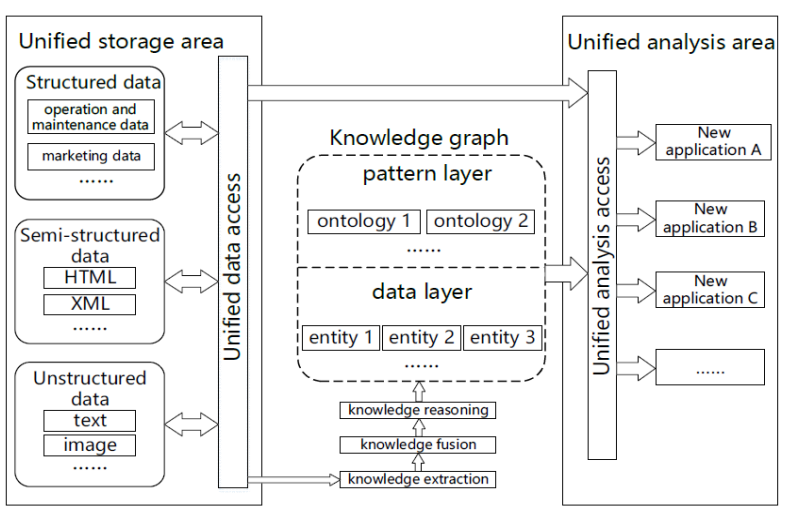
\includegraphics[width=1.00\textwidth]{images/arc-graph.png}
    \caption{Arsitektur \textit{Knowledge Graph} \parencite{yu2021visualkg}}
    \label{fig:arc-kg}
\end{figure}

\textcite{abusalih2021domain} mengklasifikasikan konstruksi KG ke dalam dua dimensi utama seperti yang bisa dilihat pada Gambar \ref{fig:tax-kg}. Dimensi pertama membagi KG berdasarkan jenis basis pengetahuan yang digunakan, yaitu \textit{schema-based}, \textit{schema-free}, dan \textit{hybrid}. Pendekatan \textit{schema-based} membangun KG berdasarkan ontologi atau skema yang telah didefinisikan sebelumnya; pendekatan \textit{schema-free} menggunakan teknik ekstraksi terbuka (\textit{Open Information Extraction}) tanpa panduan ontologi; sedangkan \textit{hybrid} menggabungkan keduanya. Dimensi kedua mengklasifikasikan metode konstruksi berdasarkan teknik yang digunakan, yaitu \textit{rule/knowledge-based} yang mengandalkan aturan eksplisit yang dirancang oleh pakar domain, \textit{learning-based} yang memanfaatkan teknik statistik dan supervised learning, pendekatan berbasis jaringan saraf (\textit{neural networks}), serta pemanfaatan alat NLP siap pakai (\textit{off-the-shelf tools}).

\begin{figure}[h]
    \centering
    \captionsetup{justification=centering}
    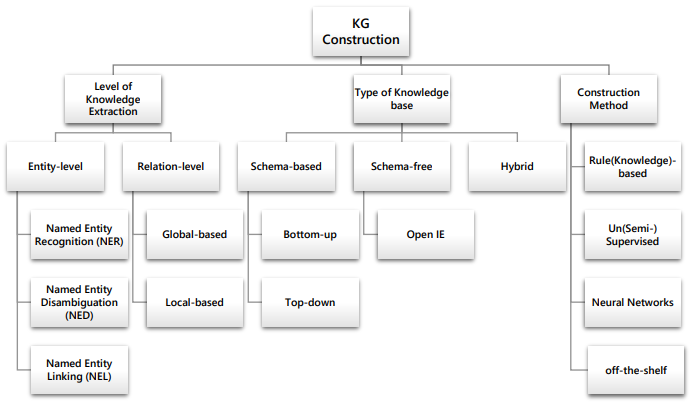
\includegraphics[width=1.00\textwidth]{images/Taxonomy-KG.png}
    \caption{Taksonomi pada pembangunan \textit{Knowledge Graph} \parencite{abusalih2021domain}}
    \label{fig:tax-kg}
\end{figure}

Posisi penelitian ini dalam taksonomi tersebut terletak pada kombinasi \textit{schema-based} dengan metode \textit{rule/knowledge-based}: sumber pengetahuan berupa spesifikasi OpenAPI Kubernetes yang bersifat formal dan terstruktur, sementara konstruksi KG dilakukan melalui aturan transformasi deterministik yang dirancang secara eksplisit berdasarkan semantik domain. Berbeda dengan pendekatan \textit{schema-free} berbasis LLM yang bersifat stokastik dan menghasilkan struktur graf yang bervariasi antareksekusi \parencite{pan2024unifying}, pendekatan \textit{rule-based} menghasilkan representasi yang konsisten dan dapat direproduksi selama sumber skemanya tidak berubah.

Sifat deterministik KG berbasis skema ini membuka peluang penggunaan ganda: selain sebagai basis \textit{retrieval}, graf yang sama dapat dimanfaatkan sebagai validator struktural. \textcite{rahman2023misconfigurations} menemukan bahwa sekitar 80\% miskonfigurasi Kubernetes bersifat struktural sehingga dapat dideteksi melalui analisis statis (\textit{static analysis}) tanpa menjalankan klaster aktif. Temuan ini memvalidasi prinsip pendekatan validasi berbasis skema: jika spesifikasi \textit{required fields} setiap objek Kubernetes sudah terenkode dalam representasi graf, pemeriksaan kelengkapan atribut wajib dapat dilakukan langsung terhadap graf tersebut, tanpa memerlukan mekanisme \textit{dry-run} yang bergantung pada infrastruktur nyata.

\subsection{GraphRAG: Integrasi \textit{Knowledge Graph} dan \textit{Large Language Models}}
\label{subsec:graphrag}

\textit{Large Language Models} (LLM) dan \textit{Knowledge Graphs} (KG) merupakan dua paradigma representasi pengetahuan yang saling melengkapi. LLM unggul dalam pemrosesan bahasa alami serta generalisasi lintas tugas, tetapi rentan terhadap halusinasi fakta. Sebaliknya, KG menawarkan representasi pengetahuan faktual dalam bentuk struktur graf eksplisit yang kuat untuk penalaran simbolik, namun kurang mampu menangani pemahaman bahasa alami yang kompleks \parencite{pan2024unifying}.

Untuk mengatasi kelemahan LLM tersebut, pendekatan \textit{Retrieval-Augmented Generation} (RAG) konvensional sering digunakan. Namun, RAG tradisional bekerja dengan cara memecah dokumen menjadi potongan teks (\textit{chunks}) independen sehingga sering kali menghilangkan informasi struktural dan relasi esensial antarentitas \parencite{ma_llm_kg_2025}. Sebagai solusi komprehensif atas keterbatasan tersebut, muncullah konsep \textit{Graph Retrieval-Augmented Generation} (GraphRAG).

Berbeda dengan pencarian semantik biasa berbasis vektor teks, GraphRAG memanfaatkan mekanisme penelusuran graf (\textit{graph traversal}) untuk mengambil konteks terstruktur secara utuh sebelum diberikan ke LLM \parencite{han_graphrag_2024}. Mekanisme ini secara langsung mengekstraksi pengetahuan relevan dari data graf dengan merangkai subgraf atau jalur relasional berdasarkan kueri pengguna \parencite{ma_llm_kg_2025}.

Secara formal, integrasi generatif ini dimodelkan sebagai fungsi yang bersyarat terhadap pengetahuan graf:
\begin{equation}
p_{\theta}(y \mid x, \mathcal{K}) = \sum_{z \in \mathcal{Z}(x, \mathcal{K})} p_{\theta}(y \mid x, z)\, p(z \mid x, \mathcal{K}),
\eqcaption{Model kondisional GraphRAG berbasis \textit{knowledge graph}}
\label{eq:rag-conditional}
\end{equation}
dengan $\mathcal{K} = \{(h, r, t) \subseteq \mathcal{E} \times \mathcal{R} \times \mathcal{E}\}$ merepresentasikan KG sebagai himpunan \textit{triples}, dan $\mathcal{Z}(x, \mathcal{K})$ merupakan himpunan subgraf atau fakta terstruktur yang ditarik dari graf berdasarkan kueri $x$. Dalam skema ini, KG bertindak sebagai ruang pengetahuan non-parametrik penyedia panduan penalaran (\textit{reasoning guidelines}), sedangkan LLM bertindak sebagai generator parametrik \parencite{ma_llm_kg_2025}.

Pendekatan GraphRAG ini menjadi sangat krusial dalam domain berskala kompleks seperti manajemen konfigurasi Kubernetes. Dengan memetakan hierarki objek dan referensi silang ke dalam graf, algoritma \textit{traversal} dapat merangkai jejak penalaran (\textit{reasoning path}) yang kohesif. Namun demikian, kedalaman \textit{traversal} menjadi faktor kritis yang memengaruhi kualitas konteks. Jika penelusuran yang dilakukan terlalu dalam, maka akan memicu \textit{information overload} karena graf yang berkembang secara eksponensial memungkinkan masuknya informasi yang tidak relevan \parencite{han_graphrag_2024}, sedangkan penelusuran yang terlalu dangkal menyebabkan \textit{under-retrieval} sehingga konteks relasional yang dibutuhkan untuk penalaran \textit{multi-hop} tidak terjangkau saat proses penelusuran graf.

Solusi atas dilema kedalaman ini adalah mekanisme \textit{intent-adaptive retrieval}, yaitu strategi yang menyesuaikan kedalaman atau strategi \textit{traversal} berdasarkan klasifikasi maksud (\textit{intent}) dari kueri pengguna. Literatur NLP dan IR menunjukkan bahwa mengklasifikasi tipe kueri sebelum \textit{retrieval} meningkatkan presisi konteks secara signifikan \parencite{zhao_rag_survey_2024}: kueri definitif (\textit{explain}) memerlukan konteks yang lebih dangkal dan terfokus, sedangkan kueri generatif atau relasional (\textit{generate\_yaml}, \textit{trace\_relationship}) memerlukan penelusuran yang lebih dalam untuk menangkap dependensi multi-tingkat antarobjek. Dengan demikian, klasifikasi \textit{intent} bukan sekadar pra-pemrosesan kueri, melainkan mekanisme kendali yang menentukan batas eksplorasi kontekstual dalam ruang graf.

\section{Metrik Evaluasi Sistem \textit{GraphRAG}}
\label{sec:metrik-evaluasi}

Evaluasi sistem \textit{GraphRAG} menggunakan kerangka tiga dimensi yang diadaptasi dari \textcite{ma_llm_kg_2025}: \textit{Answer Quality} (AnsQ), \textit{Retrieval Quality} (RetQ), dan \textit{Reasoning Quality} (ReaQ). Bagian ini membahas konsep dan formulasi tiap metrik dalam setiap dimensi. Seluruh metrik dinormalisasi ke rentang $[0,1]$ dengan orientasi seragam sehingga nilai yang lebih tinggi menandakan kualitas yang lebih baik.

Dari kerangka RAGAS \parencite{es_ragas_2023}, penelitian ini mengadopsi dua metrik: \textit{Answer Semantic Similarity} (AnsQ) dan \textit{Faithfulness} (ReaQ). Metrik RAGAS lainnya (\textit{Context Precision}, \textit{Context Recall}) tidak digunakan karena kualitas \textit{retrieval} diukur via RetQ berbasis \textit{node} mengikuti kerangka IR standar \parencite{manning_ir_2008}.

\subsection{\textit{Answer Quality} (AnsQ)}

Evaluasi dimensi kualitas jawaban mencakup kemiripan semantik jawaban terhadap \textit{ground truth} (\textit{Answer Semantic Similarity}), serta validitas struktural keluaran YAML untuk \textit{fixture} bertipe \textit{yaml\_gen}.

\begin{enumerate}
    \item \textbf{\textit{Answer Semantic Similarity} (AR)}\\
    Mengukur kemiripan semantik antara jawaban sistem dan jawaban \textit{ground truth} menggunakan kemiripan kosinus \textit{embedding} \parencite{es_ragas_2023}:
    \begin{equation}
    \text{AR} = \cos(\mathbf{e}_{\text{ans}},\, \mathbf{e}_{\text{gt}})
    = \frac{\mathbf{e}_{\text{ans}} \cdot \mathbf{e}_{\text{gt}}}{\lVert\mathbf{e}_{\text{ans}}\rVert\,\lVert\mathbf{e}_{\text{gt}}\rVert},
    \eqcaption{Metrik \textit{Answer Semantic Similarity}: kemiripan kosinus jawaban sistem dan \textit{ground truth}}
    \label{eq:answer-relevance}
    \end{equation}
    dengan $\mathbf{e}_{\text{ans}}$ adalah vektor \textit{embedding} jawaban sistem dan $\mathbf{e}_{\text{gt}}$ adalah vektor \textit{embedding} jawaban \textit{ground truth}.

    \item \textbf{\textit{Syntactic Validity}}\\
    Mengukur proporsi keluaran YAML yang dapat diurai tanpa galat menggunakan \textit{parser} \texttt{pyyaml}. Metrik ini bersifat biner pada level \textit{fixture} \parencite{moreno2025rag}:
    \begin{equation}
    \text{Syntactic Validity} = \frac{|\,\text{YAML lolos } parsing\,|}{|\,\text{total } fixture\ \textit{yaml\_gen}\,|}.
    \eqcaption{Metrik \textit{Syntactic Validity} keluaran YAML}
    \label{eq:syntactic-validity}
    \end{equation}

    \item \textbf{\textit{Schema Compliance}}\\
    Mengukur kesesuaian YAML terhadap spesifikasi OpenAPI Kubernetes v1.30 \parencite{kubernetes_docs}:
    \begin{equation}
    \text{Schema Compliance} = \frac{|\,\text{YAML lolos validasi skema}\,|}{|\,\text{total } fixture\ \textit{yaml\_gen}\,|}.
    \eqcaption{Metrik \textit{Schema Compliance} terhadap spesifikasi OpenAPI Kubernetes}
    \label{eq:schema-compliance}
    \end{equation}

\end{enumerate}

Dua metrik terakhir (\textit{Syntactic Validity}, \textit{Schema Compliance}) hanya berlaku untuk \textit{fixture} bertipe \textit{yaml\_gen}, sedangkan AR (\textit{Answer Semantic Similarity}) berlaku untuk seluruh mode sistem (GraphRAG, Vector, LLM).

\subsection{\textit{Retrieval Quality} (RetQ)}

Evaluasi dimensi kualitas \textit{retrieval} menggunakan metrik IR standar berbasis \textit{node} \parencite{manning_ir_2008}. Misalkan $N_{\text{retrieved}}$ adalah himpunan \textit{node} yang diambil dan $N_{\text{relevant}}$ adalah himpunan \textit{node} relevan menurut \textit{ground truth}.

\begin{enumerate}
    \item \textbf{Precision@k dan Recall@k}\\
    \textit{Precision@k} mengukur proporsi \textit{node} relevan di antara \textit{node} yang diambil, sedangkan \textit{Recall@k} mengukur proporsi \textit{node} relevan yang berhasil ditemukan dari seluruh \textit{node} relevan yang ada \parencite{zhao_rag_survey_2024}:
    \begin{equation}
    \text{Precision@k} = \frac{|\,N_{\text{retrieved}} \cap N_{\text{relevant}}\,|}{|\,N_{\text{retrieved}}\,|}, \qquad
    \text{Recall@k} = \frac{|\,N_{\text{retrieved}} \cap N_{\text{relevant}}\,|}{|\,N_{\text{relevant}}\,|}.
    \eqcaption{Metrik \textit{Precision@k} dan \textit{Recall@k} pada \textit{retrieval}}
    \label{eq:precision-recall}
    \end{equation}

    \item \textbf{F1-Score@k}\\
    Merupakan rata-rata harmonik antara \textit{Precision@k} dan \textit{Recall@k} \parencite{zhao_rag_survey_2024}:
    \begin{equation}
    \text{F1@k} = 2 \times \frac{\text{Precision@k} \times \text{Recall@k}}{\text{Precision@k} + \text{Recall@k}}.
    \eqcaption{Metrik \textit{F1-Score@k}: rata-rata harmonik presisi dan kelengkapan}
    \label{eq:f1}
    \end{equation}

\end{enumerate}

Metrik \textit{Precision@k}, \textit{Recall@k}, dan \textit{F1@k} hanya berlaku untuk mode GraphRAG dan Vector; mode LLM tidak melakukan \textit{retrieval} eksplisit sehingga metrik ini tidak dapat diukur.

\subsection{\textit{Reasoning Quality} (ReaQ)}

Evaluasi dimensi penalaran mengukur sejauh mana jalur \textit{multi-hop} dan ketersandaran jawaban pada konteks yang diambil. \textit{Hop-Accuracy} bersifat intrinsik graf (GraphRAG), sedangkan \textit{Faithfulness} berlaku untuk mode GraphRAG dan Vector RAG.

\begin{enumerate}
    \item \textbf{\textit{Hop-Accuracy} (Hop-Acc)}\\
    Mengukur sejauh mana jalur penalaran \textit{multi-hop} yang dieksekusi sistem mencakup relasi yang diharapkan menurut anotasi \textit{ground truth}, dalam bentuk \textit{edge recall} pada subgraf penalaran \parencite{gu_2024}:
    \begin{equation}
    \text{Hop-Acc} = \frac{|\,E_{\text{pred}} \cap E_{\text{expected}}\,|}{|\,E_{\text{expected}}\,|},
    \eqcaption{Metrik \textit{Hop-Accuracy}: \textit{edge recall} jalur penalaran \textit{multi-hop}}
    \label{eq:hop-accuracy}
    \end{equation}
    dengan $E_{\text{pred}}$ adalah himpunan \textit{edge} pada jalur penalaran yang dieksekusi sistem (dari \texttt{reasoning\_path}) dan $E_{\text{expected}}$ adalah himpunan \textit{edge} yang diharapkan menurut \textit{ground truth} (dari \texttt{expected\_path}).

    \item \textbf{\textit{Faithfulness} (FS)}\\
    Mengukur proporsi klaim dalam jawaban sistem yang dapat didukung oleh konteks yang diambil, bukan dari pengetahuan parametrik LLM \parencite{es_ragas_2023}. Jawaban didekomposisi menjadi klaim-klaim individual, lalu proporsi klaim yang dapat diinferensikan dari konteks dihitung:
    \begin{equation}
    \text{FS} = \frac{|\,C_{\text{supported}}\,|}{|\,C_{\text{total}}\,|},
    \eqcaption{Metrik \textit{Faithfulness}: proporsi klaim jawaban yang didukung konteks}
    \label{eq:faithfulness}
    \end{equation}
    dengan $C_{\text{total}}$ adalah himpunan semua klaim yang diekstrak dari jawaban sistem dan $C_{\text{supported}} = \{c \in C_{\text{total}} \mid c \text{ dapat diinferensikan dari konteks yang di-\textit{retrieve}}\}$. Metrik ini berlaku untuk mode GraphRAG dan Vector RAG.
\end{enumerate}

Dalam penelitian ini, metrik dibedakan berdasarkan cakupan penerapannya: AR (\textit{Answer Semantic Similarity}) berlaku untuk ketiga mode sistem (GraphRAG, Vector, LLM); metrik RetQ (Precision, Recall, F1) hanya bermakna untuk GraphRAG dan Vector; \textit{Hop-Accuracy} bersifat intrinsik graf (GraphRAG); dan \textit{Faithfulness} berlaku untuk GraphRAG dan Vector RAG.

\section{Penelitian Terkait}
\label{sec:penelitian-terkait}

Bagian ini merangkum tiga penelitian terdahulu yang paling relevan terhadap pendekatan yang dikembangkan dalam penelitian ini. Ketiga penelitian tersebut dipilih karena secara bersama-sama merepresentasikan perkembangan mutakhir penerapan \textit{Knowledge Graph} dan RAG pada domain teknis spesifik sehingga membentuk pijakan perbandingan langsung terhadap kontribusi yang diajukan.

\subsection{GraphRAG untuk Platform IoT Domain-Spesifik}

\textcite{civiot2025graphrag} mengembangkan mesin dialog tanya jawab berbasis GraphRAG untuk membantu pengguna mengambil informasi secara presisi dari \textit{Civil IoT Taiwan Data Service Platform}. Penelitian ini membangun \textit{Knowledge Graph} secara semi-otomatis menggunakan GPT-4.1 untuk mengekstraksi entitas dan relasi dari dokumen platform, kemudian menggunakan model Llama-3-TAIDE-LX-8B untuk menerjemahkan pertanyaan bahasa alami pengguna ke jalur kueri graf. Sistem berhasil melampaui nilai F1 sebesar 0,7 pada kueri multi-entitas dan menunjukkan efektivitas dalam menghindari halusinasi pada kasus data yang tidak tersedia.

Keterbatasan utamanya adalah \textit{Knowledge Graph} yang bersifat statis tanpa mekanisme pembaruan dinamis, serta biaya adaptasi yang tinggi untuk platform lain. Perbedaan kunci dengan penelitian ini terletak pada sumber data dan topologi graf: penelitian \textcite{civiot2025graphrag} membangun graf dari narasi dokumen tidak terstruktur dengan entitas IoT yang beragam, sedangkan penelitian ini membangun graf dari skema OpenAPI Kubernetes yang bersifat deterministik dengan taksonomi relasi yang didefinisikan secara eksplisit.

\subsection{RAG Hibrida KG-Vektor untuk Manufaktur Pintar}

\textcite{wan2025empowering} mengusulkan kerangka kerja Q\&A berbasis RAG hibrida yang menggabungkan \textit{Knowledge Graph} Neo4j dengan pencarian vektor untuk domain \textit{Design for Additive Manufacturing} (DfAM). Konstruksi KG dilakukan berdasarkan metadata dari 69 publikasi teknis, diperkuat dengan \textit{Semantic Alignment} dan \textit{Prompt Enhancement} (PE) berbasis konstrain domain. Kombinasi pendekatan hibrida tersebut dengan GPT-4o menghasilkan akurasi 77,8\% \textit{Exact Match} dan 76,5\% \textit{Context Precision}, melampaui pendekatan RAG vektor atau graf secara mandiri.

Keterbatasan utamanya adalah latensi tinggi akibat proses pencarian hibrida yang kompleks, serta KG yang belum mendukung pembaruan data secara dinamis. Penelitian ini mengadopsi konsep hibrida KG-vektor yang sama, namun memperluas mekanisme \textit{retrieval} dengan pencocokan eksak berbasis nama \textit{resource} dan penelusuran multi-hop mengikuti taksonomi 18 jenis relasi Kubernetes yang dirancang secara domain-spesifik.

\subsection{HSG-RAG: Konstruksi Basis Pengetahuan Hierarkis untuk Domain Teknis}

\textcite{hsgrag2025acm} mengembangkan HSG-RAG (\textit{Hierarchical Semantic Graph Retrieval Augmented Generation}), sebuah metode konstruksi dan pencarian basis pengetahuan bertingkat untuk mendukung pengembangan sistem \textit{embedded}. Graf dibangun dari korpus dokumen teknis SDK dan \textit{datasheet} tiga platform perangkat keras (ESP32S3, STM32F103, JL701) menggunakan LLM, mencakup dua lapisan relasi: jarak dekat antarparagraf dan jarak jauh berbasis kemiripan semantik. Strategi pencarian \textit{top-down} memecah kueri pengguna menjadi sub-kueri yang ditelusuri secara bertahap di dalam graf, menghasilkan jawaban yang lebih spesifik, ringkas, dan lengkap dibandingkan VanillaRAG maupun GraphRAG konvensional.

Keterbatasan utamanya adalah belum adanya mekanisme verifikasi otomatis kebenaran kode yang dihasilkan, serta cakupan evaluasi yang masih terbatas pada beberapa platform perangkat keras. Penelitian ini mengadopsi konsep dekomposisi kueri dan penelusuran bertingkat yang serupa, namun menerapkannya pada skema Kubernetes yang memiliki hierarki objek lebih terstruktur dan jenis relasi antar\textit{resource} yang terdefinisi secara formal dalam spesifikasi OpenAPI.

Ketiga penelitian terdahulu secara konsisten memvalidasi efektivitas pendekatan GraphRAG dalam domain teknis spesifik, sekaligus mengidentifikasi dua pola keterbatasan yang berulang: (1) KG bersifat statis tanpa mekanisme pembaruan dinamis, dan (2) taksonomi relasi yang belum disesuaikan dengan karakteristik skema target secara mendalam. Penelitian ini merespons kedua pola keterbatasan tersebut secara domain-spesifik untuk Kubernetes.

Berdasarkan kajian literatur yang telah dipaparkan, teridentifikasi dua kesenjangan utama yang menjadi landasan penelitian ini. Pertama, pendekatan RAG berbasis vektor konvensional menunjukkan keterbatasan signifikan untuk domain Kubernetes karena gagal menangkap relasi hierarkis dan referensial yang menentukan validitas konfigurasi \parencite{wan2025empowering}. Kedua, meskipun integrasi \textit{Knowledge Graph} dalam RAG telah menunjukkan peningkatan signifikan pada domain umum, belum ada rancangan taksonomi relasi dan mekanisme \textit{traversal} yang secara spesifik disesuaikan untuk skema OpenAPI Kubernetes. Bab selanjutnya menganalisis karakteristik data, kebutuhan sistem, dan alternatif pendekatan solusi untuk menjawab kedua kesenjangan tersebut.
